\documentclass[border=10pt]{standalone}
\usepackage{tikz}
\usepackage{tkz-fct}
\renewcommand*\familydefault{\sfdefault}
\usepackage{sansmath}
\usepackage{amsmath}
\sansmath
\usepackage{tkz-euclide}

\begin{document}

    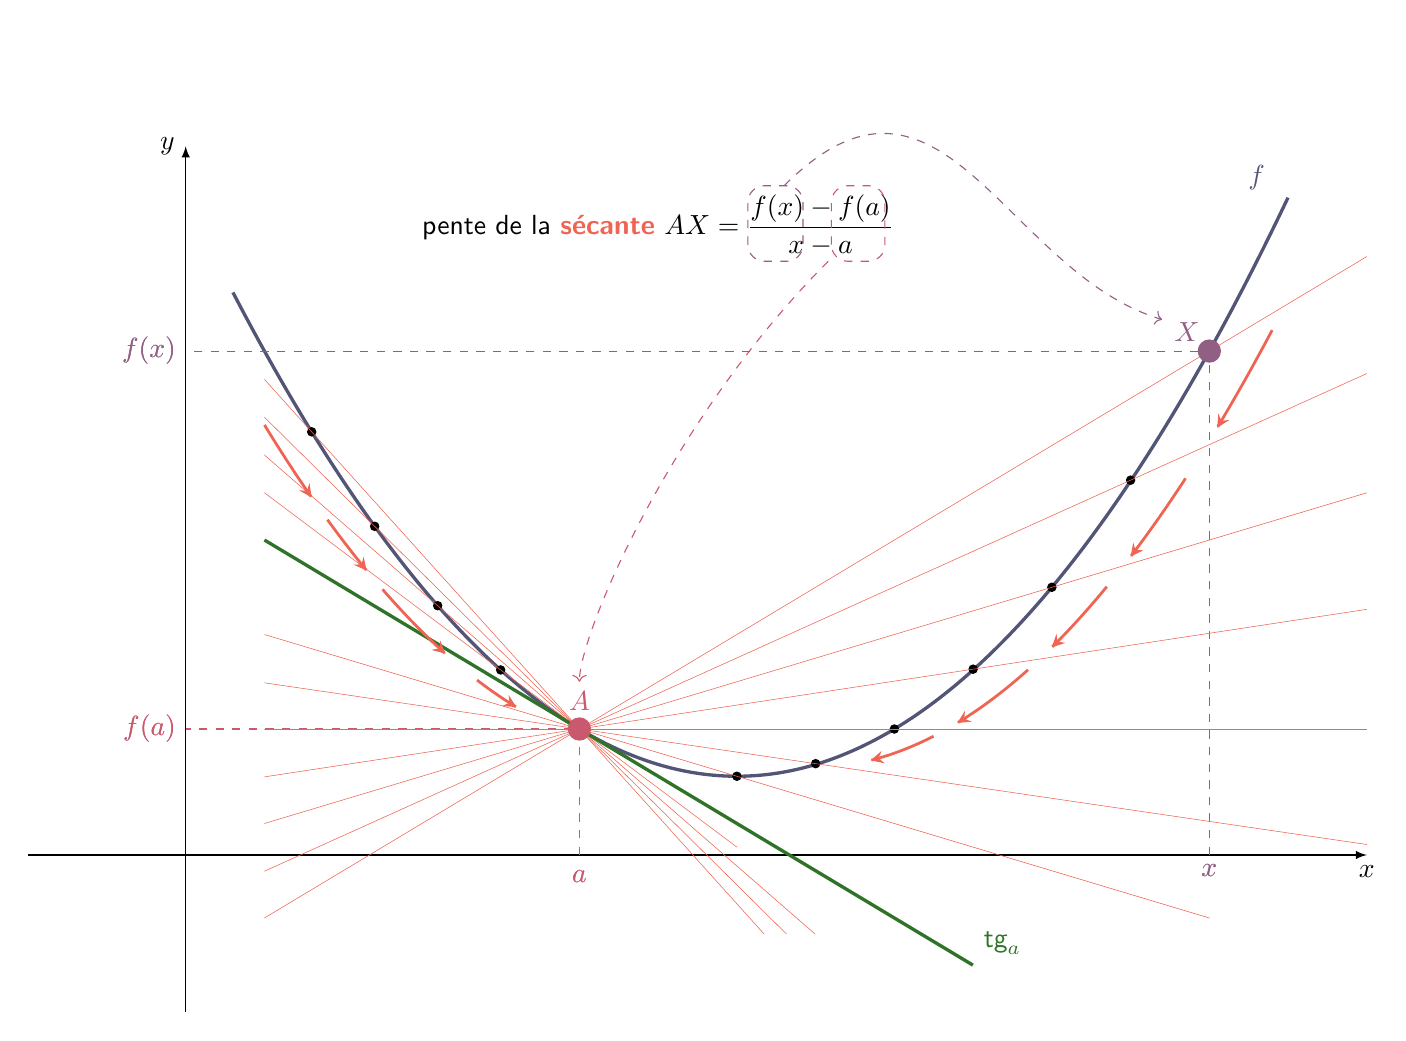
\begin{tikzpicture}[scale=2]
   \tkzInit[xmax=7.0,ymax=4.0,xmin=-1.0 ,ymin=-1.0, ystep=1]

   \tkzDrawX[noticks,label={$x$}]
   \tkzDrawY[noticks,label={$y$}]
\definecolor{ored}{cmyk}{0.0,0.63,0.62,0.02}
\definecolor{opink}{cmyk}{0.,0.59,0.32,0.2}
\definecolor{ob}{cmyk}{0.45,0.34,0.,0.49}
\definecolor{ogreen}{cmyk}{0.7,0.,0.92,0.44}
\definecolor{op}{cmyk}{0.11,0.41,0.,0.4}
  

 %\node at (3,-1) {pente de la {\bf\color{ogreen}{tangente}} au point $A=f'(a)=\lim\limits_{x\to a}\dfrac{f(x)-f(a)}{x-a}$};
\def\xA{2.5} \def\yA{0.8}
        \coordinate (A) at (\xA,\yA);
        \draw[dashed, color=opink] (\xA,0) node[below=2pt] {$a$} -- (A) -- (0,\yA) node[left] {$f(a)$};

        \def\xM{6.5} \def\yM{3.2}
        \coordinate (B) at (\xM,\yM);
        \draw[dashed, color=op] (\xM,0) node[below] {$x$} -- (B) -- (0,\yM) node[left] {$f(x)$};
  \begin{scope}[xshift=3cm, yshift= 4cm]
  \node at (0,0) {pente de la {\bf\color{ored}{sécante}} $AX=\dfrac{f(x)-f(a)}{x-a}$};
\draw[rounded corners=6pt, dashed, color=op]
    (.57,-0.23) rectangle (0.92,0.25);
\draw[rounded corners=6pt, dashed, color=opink]
    (1.1,-0.23) rectangle (1.44,0.25);
  \end{scope}
  
\draw[->, color=op, dashed]
    (3.8,4.25) .. controls +(1,1) and +(-1,0.3) .. (6.2,3.4);
\draw[->, color=opink, dashed]
    (4.08,3.77) .. controls +(-1,-1) and +(0,0.3) .. (2.5,1.1);
%\draw[step=1cm, gray!30, very thin] (-1,-1) grid (7,5);
        % Function curve
        \begin{scope}
            \clip (-1,0) rectangle (7.5,4.5);
            \draw[line width=1.2pt,color=ob,smooth,samples=100,domain=0.3:7] plot(\x,{0.3*((\x)-3.5)*((\x)-3.5)+0.5});
              \node at (6.8,4.3) {{\bf\color{ob}{$f$}}};

        \end{scope}

        \def\xA{2.5} \def\yA{0.8}
        \coordinate (A) at (\xA,\yA);
        \draw[dashed, color=opink] (\xA,0) node[below=2pt] {$a$} -- (A) -- (0,\yA) node[left] {$f(a)$};

        \def\xM{6.5} \def\yM{3.2}
        \coordinate (B) at (\xM,\yM);
        \draw[dashed, color=op] (\xM,0) node[below] {$x$} -- (B) -- (0,\yM) node[left] {$f(x)$};
        \begin{scope}
            \clip (0.5,-0.5) rectangle (7.5,4.5);

            % Series of lines all through point A
            \foreach \xN/\yN in {6.5/3.2,6/2.38,5.5/1.7,5/1.18,4.5/0.8,4/0.58,3.5/0.5,2/1.175,1.6/1.583,1.2/2.087,0.8/2.687}
                {
                \coordinate (N) at (\xN,\yN);
                \tkzDrawPoint[size=3](N)
                \tkzDrawLine[add=2 and 3,color=ored](A,N)
                }
        \end{scope}

        \draw[line
        width=1.2pt,color=ogreen,smooth,samples=100,domain=0.5:5]
        plot(\x,{-0.6*(\x)+2.3}) node[above right] {$\text{tg}_{a}$};

        \tkzDrawPoints[size=8, color=op](B)
        \tkzDrawPoints[size=8, color=opink](A)

        \tkzLabelPoint[above=3pt, color=opink](A){$A$}
        \tkzLabelPoint[above left, color=op](B){$X$}

        %%%%Arrows alongside the curve
        \foreach \a/\b in {6.55/6.9, 6/6.35, 5.5/5.85, 4.9/5.35, 4.35/4.75}
            {
            \draw[<-,>=stealth,line width=1pt,color=ored,smooth,samples=100,domain=\a:\b] plot(\x,{0.32*((\x)-3.95)*((\x)-3.95)+0.55});
            }
        \foreach \a/\b in {1.85/2.1,1.25/1.65,0.9/1.15,0.5/0.8}
            {
            \draw[->,>=stealth,line width=1pt,color=ored,smooth,samples=100,domain=\a:\b] plot(\x,{0.32*((\x)-3.05)*((\x)-3.05)+0.65});
            }

    \end{tikzpicture}
\end{document}